\iffalse
\let\negmedspace\undefined
\let\negthickspace\undefined
\documentclass[journal,12pt,onecolumn]{IEEEtran}
\usepackage{cite}
\usepackage{amsmath,amssymb,amsfonts,amsthm}
%\usepackage{algorithmic}
\usepackage{graphicx}
\usepackage{textcomp}
\usepackage{array}
\usepackage{xcolor}
\usepackage{txfonts}
\usepackage{listings}
\usepackage{enumitem}
\usepackage{mathtools}
\usepackage{gensymb}
\usepackage[breaklinks=true]{hyperref}
\usepackage{tkz-euclide} % loads  TikZ and tkz-base
\usepackage{listings}
\usepackage{float}
\usepackage{bm}



\newtheorem{theorem}{Theorem}[section]
\newtheorem{problem}{Problem}
\newtheorem{proposition}{Proposition}[section]
\newtheorem{lemma}{Lemma}[section]
\newtheorem{corollary}[theorem]{Corollary}
\newtheorem{example}{Example}[section]
\newtheorem{definition}[problem]{Definition}
%\newtheorem{thm}{Theorem}[section] 
%\newtheorem{defn}[thm]{Definition}
%\newtheorem{algorithm}{Algorithm}[section]
%\newtheorem{cor}{Corollary}
\newcommand{\BEQA}{\begin{eqnarray}}
\newcommand{\EEQA}{\end{eqnarray}}
\newcommand{\define}{\stackrel{\triangle}{=}}
\theoremstyle{remark}
\newtheorem{rem}{Remark}
%\bibliographystyle{ieeetr}
\begin{document}
%
\providecommand{\pr}[1]{\ensuremath{\Pr\left(#1\right)}}
\providecommand{\prt}[2]{\ensuremath{p_{#1}^{\left(#2\right)} }}        % own macro for this question
\providecommand{\qfunc}[1]{\ensuremath{Q\left(#1\right)}}
\providecommand{\sbrak}[1]{\ensuremath{{}\left[#1\right]}}
\providecommand{\lsbrak}[1]{\ensuremath{{}\left[#1\right.}}
\providecommand{\rsbrak}[1]{\ensuremath{{}\left.#1\right]}}
\providecommand{\brak}[1]{\ensuremath{\left(#1\right)}}
\providecommand{\lbrak}[1]{\ensuremath{\left(#1\right.}}
\providecommand{\rbrak}[1]{\ensuremath{\left.#1\right)}}
\providecommand{\cbrak}[1]{\ensuremath{\left\{#1\right\}}}
\providecommand{\lcbrak}[1]{\ensuremath{\left\{#1\right.}}
\providecommand{\rcbrak}[1]{\ensuremath{\left.#1\right\}}}
\newcommand{\sgn}{\mathop{\mathrm{sgn}}}
\providecommand{\abs}[1]{\left\vert#1\right\vert}
\providecommand{\res}[1]{\Res\displaylimits_{#1}} 
\providecommand{\norm}[1]{\left\lVert#1\right\rVert}
%\providecommand{\norm}[1]{\lVert#1\rVert}
\providecommand{\mtx}[1]{\mathbf{#1}}
\providecommand{\mean}[1]{E\left[ #1 \right]}
\providecommand{\cond}[2]{#1\middle|#2}
\providecommand{\fourier}{\overset{\mathcal{F}}{ \rightleftharpoons}}
\newenvironment{amatrix}[1]{%
  \left(\begin{array}{@{}*{#1}{c}|c@{}}
}{%
  \end{array}\right)
}
%\providecommand{\hilbert}{\overset{\mathcal{H}}{ \rightleftharpoons}}
%\providecommand{\system}{\overset{\mathcal{H}}{ \longleftrightarrow}}
	%\newcommand{\solution}[2]{\textbf{Solution:}{#1}}
\newcommand{\solution}{\noindent \textbf{Solution: }}
\newcommand{\cosec}{\,\text{cosec}\,}
\providecommand{\dec}[2]{\ensuremath{\overset{#1}{\underset{#2}{\gtrless}}}}
\newcommand{\myvec}[1]{\ensuremath{\begin{pmatrix}#1\end{pmatrix}}}
\newcommand{\mydet}[1]{\ensuremath{\begin{vmatrix}#1\end{vmatrix}}}
\newcommand{\myaugvec}[2]{\ensuremath{\begin{amatrix}{#1}#2\end{amatrix}}}
\providecommand{\rank}{\text{rank}}
\providecommand{\pr}[1]{\ensuremath{\Pr\left(#1\right)}}
\providecommand{\qfunc}[1]{\ensuremath{Q\left(#1\right)}}
	\newcommand*{\permcomb}[4][0mu]{{{}^{#3}\mkern#1#2_{#4}}}
\newcommand*{\perm}[1][-3mu]{\permcomb[#1]{P}}
\newcommand*{\comb}[1][-1mu]{\permcomb[#1]{C}}
\providecommand{\qfunc}[1]{\ensuremath{Q\left(#1\right)}}
\providecommand{\gauss}[2]{\mathcal{N}\ensuremath{\left(#1,#2\right)}}
\providecommand{\diff}[2]{\ensuremath{\frac{d{#1}}{d{#2}}}}
\providecommand{\myceil}[1]{\left \lceil #1 \right \rceil }
\newcommand\figref{Fig.~\ref}
\newcommand\tabref{Table~\ref}
\newcommand{\sinc}{\,\text{sinc}\,}
\newcommand{\rect}{\,\text{rect}\,}
%%
%	%\newcommand{\solution}[2]{\textbf{Solution:}{#1}}
%\newcommand{\solution}{\noindent \textbf{Solution: }}
%\newcommand{\cosec}{\,\text{cosec}\,}
%\numberwithin{equation}{section}
%\numberwithin{equation}{subsection}
%\numberwithin{problem}{section}
%\numberwithin{definition}{section}
%\makeatletter
%\@addtoreset{figure}{problem}
%\makeatother

%\let\StandardTheFigure\thefigure
\let\vec\mathbf

\bibliographystyle{IEEEtran}





\bigskip

%\renewcommand{\thefigure}{\theenumi}
%\renewcommand{\thetable}{\theenumi}
%\renewcommand{\theequation}{\theenumi}

Q:  The block diagram of a two-tap high-pass FIR filter is shown below. The filter transfer function is given by $H(z) = Y(z)/X(z)$.\\
If the ratio of maximum to minimum value of $H(z)$ is 2 and $\abs{H(z)}_{max} = 1$, the coefficients $\beta_0$ and $\beta_1$ are \underline{\hspace{3cm}} and \underline{\hspace{3cm}}, respectively. 

\begin{figure}[H]
    \centering
    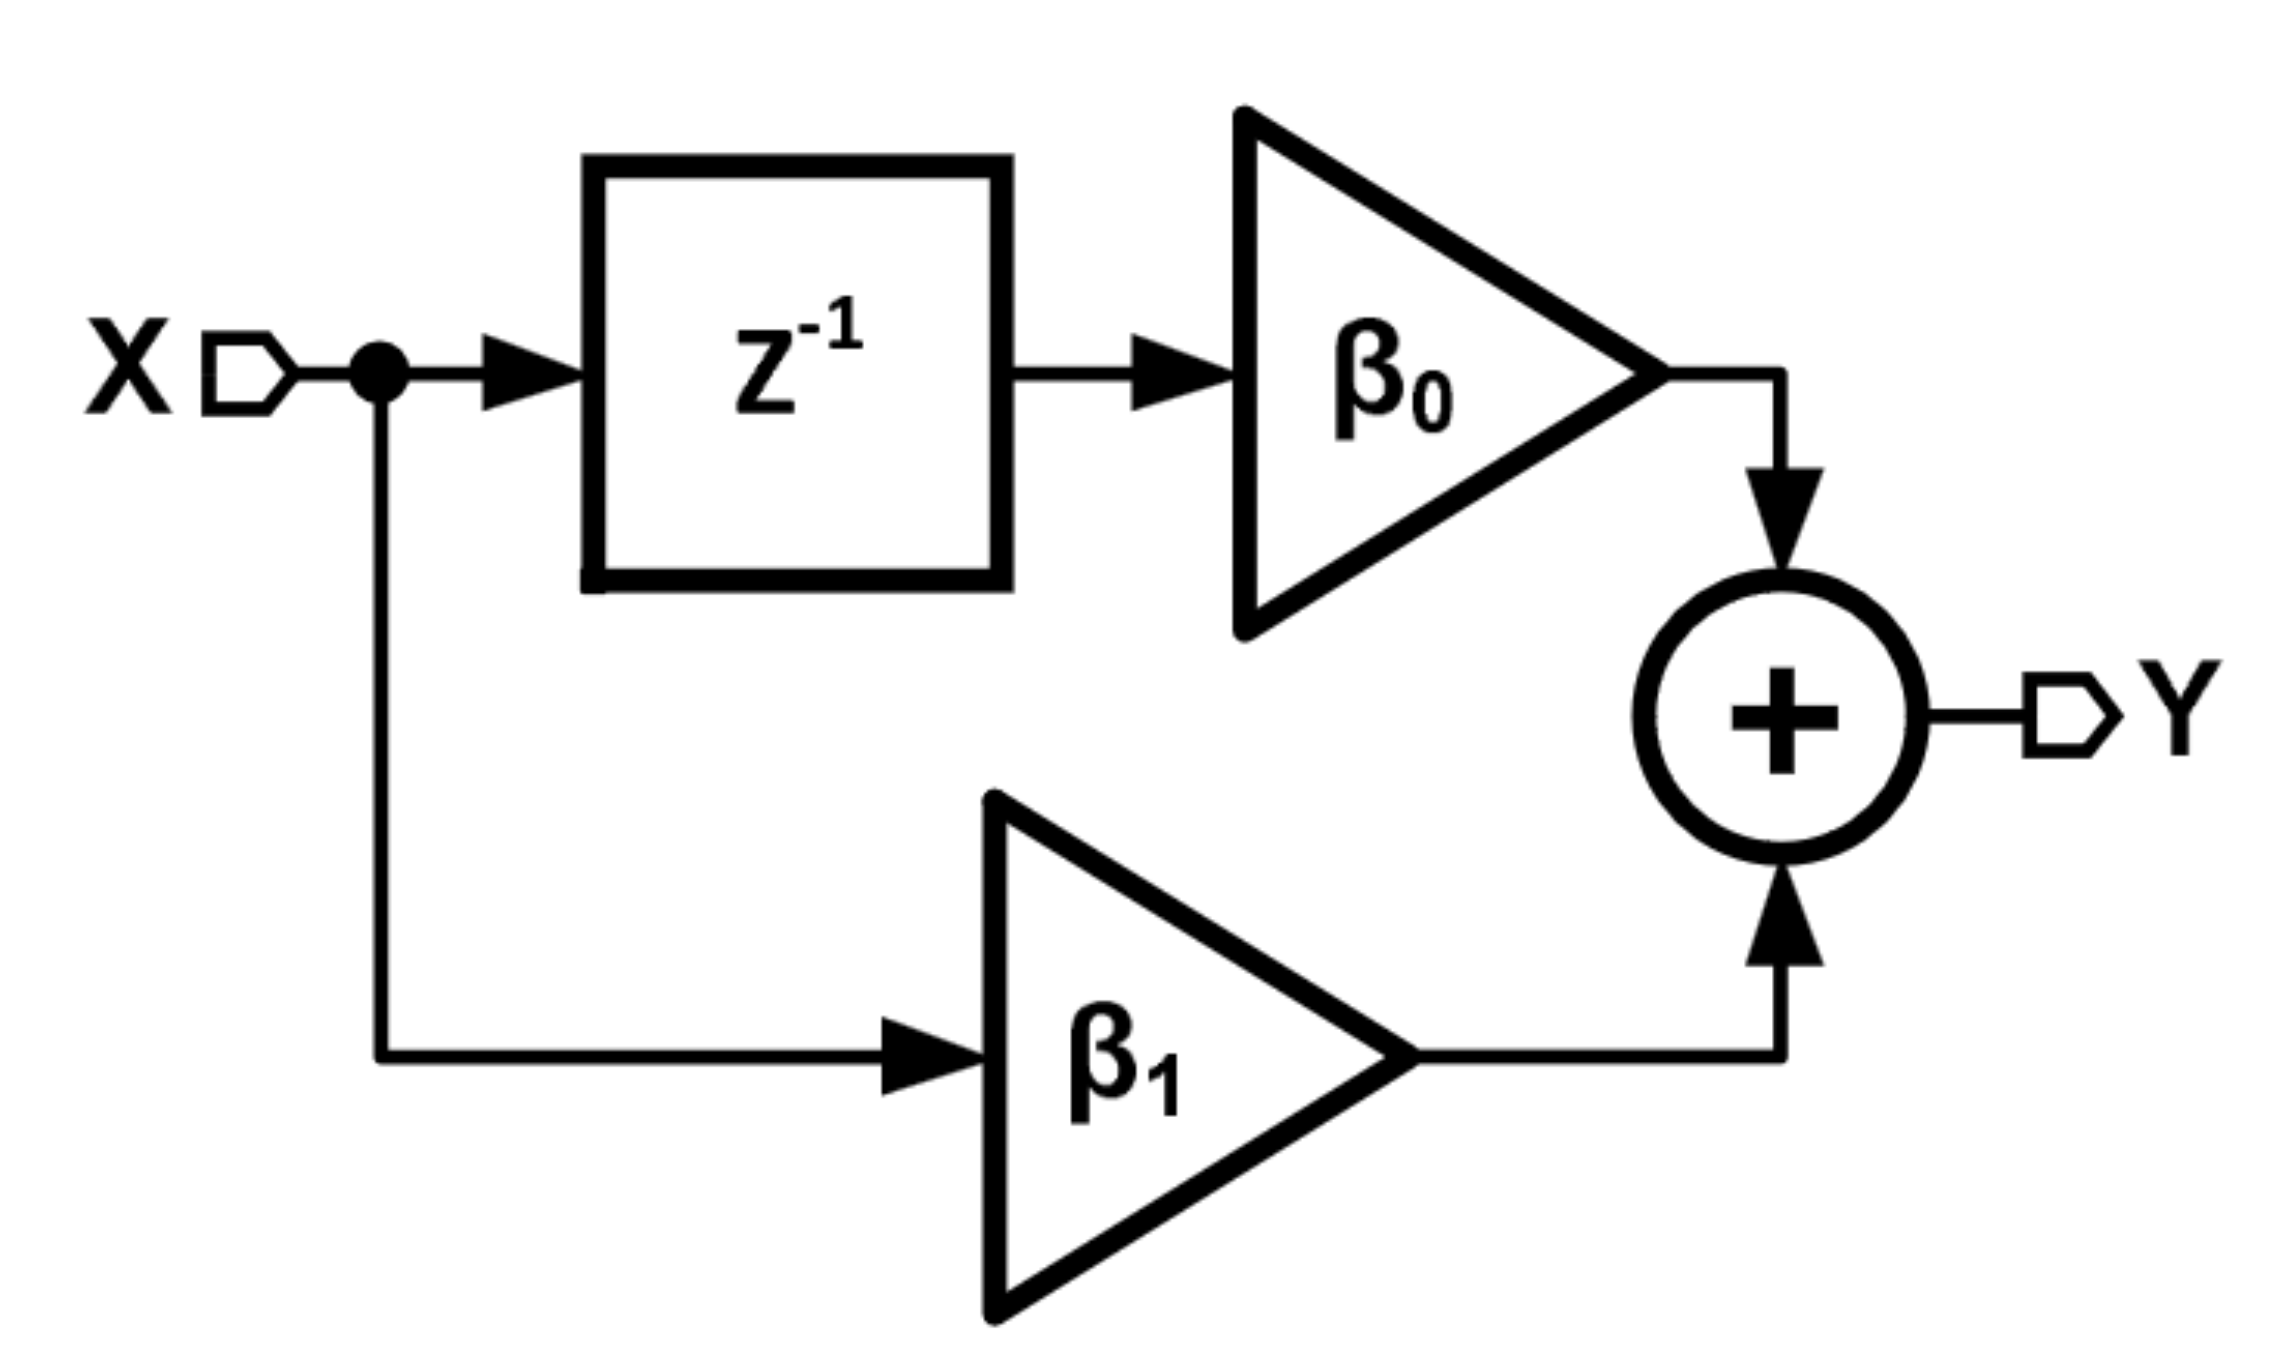
\includegraphics[width=0.5\linewidth]{2022/BM/39/figs/qfig.png} 
    \caption{Block diagram}
    \label{fig:GATE22BM39.1}
\end{figure}


\begin{enumerate}[label=(\Alph*)]
\item 0.75, -0.25
\item 0.67, 0.33
\item 0.60, -0.40
\item -0.64, 0.36
\end{enumerate}
\hfill{GATE BM 2022}


\solution \\
\fi
\textbf{Results and Proofs: \\}
\underline{Time Shift Property:}
\begin{align}
x(n) &\overset{\mathcal{Z}}{\longleftrightarrow} X(z) \\
x(n-n_0) &\overset{\mathcal{Z}}{\longleftrightarrow} z^{-n_0}X(z) 
\end{align}
\underline{Proof:} \\
Let
\begin{align}
y(n) &= x(n-n_0) \label{eq:GATE22BM39.-1}
\end{align}
Taking z-transform
\begin{align}
\mathcal{Z}\brak{y(n)} &= \mathcal{Z}\brak{x(n-n_0)} \label{eq:GATE22BM39.-2}\\
\end{align}
Simplifying LHS
\begin{align}
Y(z) &= \sum_{n=-\infty}^{\infty} y(n)z^{-n} 
\end{align}
From \eqref{eq:GATE22BM39.-1}
\begin{align}
Y(z) &= \sum_{n=-\infty}^{\infty} x(n-n_0) z^{-n} \label{eq:GATE22BM39.-3}
\end{align}
Let 
\begin{align}
n-n_0 &= s  \\\implies
n &= s+n_0 \label{eq:GATE22BM39.-4}
\end{align}
From \eqref{eq:GATE22BM39.-3} and \eqref{eq:GATE22BM39.-4}
\begin{align}
Y(z) &= \sum_{s=-\infty}^{\infty} x(s) z^{-(s+n_0)} \\
&= z^{-n_0}\sum_{s=-\infty}^{\infty} x(s) z^{-s} 
\end{align}
As variable in Z-transform is dummy, on replacing it, we get
\begin{align}
Y(z) &= z^{-n_0}\sum_{n=-\infty}^{\infty} x(n) z^{-n} \\
&= z^{-n_0}X(z) \label{eq:GATE22BM39.-5}
\end{align}
From \eqref{eq:GATE22BM39.-2} and \eqref{eq:GATE22BM39.-5}
\begin{align}
\mathcal{Z}\brak{x(n-n_0)} &= z^{-n_0}X(z)
\end{align}
Hence proved \\
\underline{Result:}
\begin{align}
z^{-n_0}X(z) &\overset{\mathcal{Z^{-}}}{\longleftrightarrow} x(n-n_0) \label{eq:GATE22BM39.-6}
\end{align}
\textbf{Sol:  }
\begin{table}[h]
    \centering
        \begin{tabular}{|c|c|c|} 
      \hline
\textbf{Variable}& \textbf{Description}& \textbf{Value}\\\hline
	 $H(z)$ & Transfer Function & $\beta_0z^{-1} + \beta_1$ \\\hline
         $\abs{H(z)}_{max}$ & Maximum value of Transfer Function & 1 \\\hline  
         $\abs{H(z)}_{min}$ & Minimum value of Transfer Function & $\frac{1}{2}$\\\hline
    \end{tabular}

    \caption{input parameters}
    \label{tab:GATE22BM39.1}
\end{table}
\\In \eqref{eq:GATE22BM39.-6}, put
\begin{align}
n_0 = 1, \quad x(n) = \delta(n) \nonumber 
\end{align}
Since
\begin{align}
1 \overset{\mathcal{Z^{-}}}{\longleftrightarrow} \delta(n) \nonumber
\end{align}
\begin{align}
z^{-1} &\overset{\mathcal{Z^{-}}}{\longleftrightarrow} \delta(n-1)
\end{align}
This is a unit delay in discrete time and represents unit amplitude sinosoidal signal.\\
So,
\begin{align}
z^{-1} &= e^{-jw} \\\implies
\abs{z^{-1}} &= 1 \label{eq:GATE22BM39.1}
\end{align}
Since $H(z)$ is complex, on using Triangle Inequality, we get
\begin{align}
\abs{x + y} \leq \abs{x} + \abs{y} 
\end{align}
And its corollary
\begin{align}
\abs{\abs{x}-\abs{y}} \leq \abs{x + y}
\end{align}
where x and y are complex numbers.
\begin{align}
\abs{\abs{z^{-1}\beta_0}-\abs{\beta_1}} \leq \abs{z^{-1}\beta_0 + \beta_1} \leq \abs{z^{-1}\beta_0} + \abs{\beta_1} 
\end{align}
From \tabref{tab:GATE22BM39.1}
\begin{align}
\abs{\abs{z^{-1}\beta_0}-\abs{\beta_1}} \leq \abs{H(z)} \leq \abs{z^{-1}\beta_0} + \abs{\beta_1}
\end{align}
From \eqref{eq:GATE22BM39.1} 
\begin{align}
\abs{\abs{\beta_0}-\abs{\beta_1}} \leq \abs{H(z)} \leq \abs{\beta_0} + \abs{\beta_1} 
\end{align}
So, we can conclude that
\begin{align}
\abs{H(z)}_{max} &= \abs{\beta_0} + \abs{\beta_1} 
\end{align}
Now from \tabref{tab:GATE22BM39.1}
\begin{align}
1 &= \abs{\beta_0} + \abs{\beta_1} \label {eq:GATE22BM39.2}
\end{align}
Similarly,
\begin{align}
\frac{1}{2} &= \abs{\abs{\beta_0}-\abs{\beta_1}} \label {eq:GATE22BM39.3}
\end{align}
On solving \eqref{eq:GATE22BM39.2} and \eqref{eq:GATE22BM39.3}, we get
\begin{align}
\abs{\beta_0} = 0.75, \abs{\beta_1} = 0.25 
\end{align}
\begin{center}
OR
\end{center}
\begin{align}
\abs{\beta_0} = 0.25, \abs{\beta_1} = 0.75 
\end{align}
Hence the correct answer is option (A) \\




%\end{document}
